\newcommand{\lecturetitle}{Practical Training of Deep Networks}
\newcommand{\lecturesubtitle}{Normalisation, stabilisation, and diagnosis}
\newcommand{\covertext}{Make\\training\\work}

% Shared preamble for new AICE3002/AICE6001 lecture decks.
% Define \lecturetitle, \lecturesubtitle and \covertext before including this file.

\ifdefined\beamerclass
\else
  \def\beamerclass{beamer}
\fi

\ifdefined\articlemode
  \documentclass[]{article}
  \usepackage[a4paper,margin=2cm]{geometry}
  \usepackage[envcountsect]{beamerarticle}
  \usepackage{parskip}
  \usepackage[hidelinks]{hyperref}
\else
  \documentclass[\beamerclass,ignorenonframetext]{beamer}
\fi

\usepackage{pgfpages}
\mode<handout>{
  \pgfpagesuselayout{2 on 1}[a4paper,border shrink=5mm]
}

\usepackage{lmodern}
\usepackage[english]{babel}
\usepackage[utf8]{inputenc}
\usepackage{amsmath}
\usepackage{bm}
\usepackage{graphicx}
\usepackage{hyperref}
\usepackage{tikz}

\usetheme{Copenhagen}
\useoutertheme{infolines}
\setbeamertemplate{headline}{}
\setbeamertemplate{navigation symbols}{}
\hypersetup{pdfstartview={Fit}}

\definecolor{darkblue}{RGB}{37,55,97}
\definecolor{mellowyellow}{RGB}{247,206,70}

\title[AICE3002 / AICE6001]{\lecturetitle}
\subtitle{\lecturesubtitle}
\author{Jonathon Hare and Antonia Marcu}
\institute[]{
  Vision, Learning and Control\\
  University of Southampton
}
\date{}
\subject{Computer Science}

\begin{document}
\mode<article>{\maketitle}

\mode<presentation>{
  \begin{frame}[plain]
    \begin{tikzpicture}[
      overlay,
      remember picture,
      shift={(current page.south west)},
      font={\fontfamily{Montserrat-TOsF}\selectfont}
    ]
      \fill[mellowyellow] (0,0) rectangle (\paperwidth,\paperheight);
      \node[
        anchor=west,
        align=left,
        text=darkblue
      ] at (1.5,5.6) {\Huge\bfseries \begin{tabular}{l}\covertext\end{tabular}};
      \node[anchor=east] at (12.3,1.0) {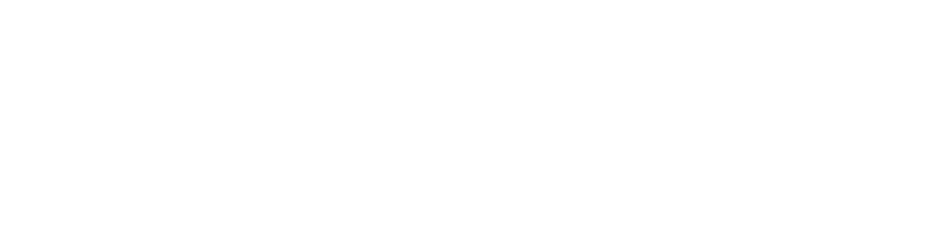
\includegraphics[scale=0.15]{../vlc.png}};
    \end{tikzpicture}
  \end{frame}
}

\begin{frame}
  \titlepage
\end{frame}


%-------------------------------------------------------------

\begin{frame}{Topics}
\begin{itemize}
  \item Initialisation, normalisation, and residual pathways
  \item Gradient clipping, learning-rate schedules, and weight decay
  \item Reading training curves and inspecting internal signals
  \item A systematic workflow for diagnosing failed training runs
\end{itemize}
\end{frame}

%-------------------------------------------------------------

\begin{frame}{Training is a coupled dynamical system}
For parameters $\bm\theta_t$, an optimiser produces an update
\[
  \bm\theta_{t+1}
  = \bm\theta_t + \Delta\bm\theta_t,
  \qquad
  \Delta\bm\theta_t
  = \operatorname{update}(\nabla_{\bm\theta}\mathcal L_t,
                           \text{optimiser state}).
\]

\begin{itemize}
  \item The gradient depends on the data, architecture, current parameters, loss, and numerical precision.
  \item The effect of the gradient depends on the optimiser, learning rate, and parameter scale.
  \item A symptom such as a flat loss curve therefore has several possible causes.
\end{itemize}

\begin{block}{The practical question}
What evidence would distinguish the possible causes?
\end{block}
\end{frame}

%-------------------------------------------------------------

\begin{frame}{Sanity checks before a long training run}
\begin{itemize}
  \item Inspect a minibatch: shapes, dtypes, value ranges, targets, and class frequencies.
  \item Check the contract between the model output and the loss. For example,
  \texttt{CrossEntropyLoss} expects raw logits and integer class indices.
  \item Verify that every intended parameter receives a finite gradient.
  \item Disable augmentation and regularisation, then overfit one small minibatch.
  \begin{itemize}
    \item Failure usually points to the implementation, optimisation, or data pipeline rather than generalisation.
  \end{itemize}
  \item Compare against a simple baseline before investing in a large run.
\end{itemize}
\end{frame}

%-------------------------------------------------------------

\begin{frame}{Initialisation recap}
\begin{itemize}
  \item Random weights break symmetry between units.
  \item Their scale should match the activation and the layer's fan-in and fan-out.
\end{itemize}

\begin{center}
\begin{tabular}{lll}
\hline
Activation & Typical choice & Weight variance \\
\hline
Linear or tanh & Xavier / Glorot & $2/(n_{\mathrm{in}}+n_{\mathrm{out}})$ \\
ReLU & He / Kaiming & $2/n_{\mathrm{in}}$ \\
\hline
\end{tabular}
\end{center}

\begin{itemize}
  \item Sensible initialisation keeps early activations and gradients at a useful scale.
  \item It only controls the start of training. Parameter updates can still move the network into a poorly scaled regime.
  \item PyTorch's historical \texttt{nn.Linear} default is not the standard He initialisation for ReLU.
\end{itemize}
\end{frame}

%-------------------------------------------------------------

\begin{frame}{Normalisation controls activation scale}
Suppose a layer produces pre-activations $\bm z$. A normalisation layer constructs
\[
  \hat{\bm z}
  = \frac{\bm z-\bm\mu}{\sqrt{\bm\sigma^2+\epsilon}},
  \qquad
  \bm y=\bm\gamma\odot\hat{\bm z}+\bm\beta.
\]

\begin{itemize}
  \item The choice of axes used to compute $\bm\mu$ and $\bm\sigma^2$ defines the normalisation method.
  \item The learned scale $\bm\gamma$ and shift $\bm\beta$ allow the layer to recover a useful representation.
  \item Normalisation changes the optimisation problem. It does not merely standardise the final representation.
  \item The small constant $\epsilon$ prevents division by zero and affects numerical behaviour when the variance is tiny.
\end{itemize}
\end{frame}

%-------------------------------------------------------------

\begin{frame}{Batch normalisation}
For feature or channel $k$ and a minibatch containing $m$ values:
\[
  \mu_k=\frac{1}{m}\sum_{i=1}^{m}z_{ik},
  \qquad
  \sigma_k^2=\frac{1}{m}\sum_{i=1}^{m}(z_{ik}-\mu_k)^2,
\]
\[
  y_{ik}=\gamma_k
  \frac{z_{ik}-\mu_k}{\sqrt{\sigma_k^2+\epsilon}}+\beta_k.
\]

\begin{itemize}
  \item For a fully connected layer, statistics are normally computed over the batch for each feature.
  \item For a convolutional layer, they are normally computed over the batch and spatial positions for each channel.
  \item Each example therefore influences the normalised representation of the other examples in its minibatch.
\end{itemize}
\end{frame}

%-------------------------------------------------------------

\begin{frame}{BatchNorm during training and evaluation}
\begin{columns}[T]
\begin{column}{0.47\textwidth}
\textbf{Training mode}
\begin{itemize}
  \item Normalises using the current minibatch statistics.
  \item Updates running estimates of the mean and variance.
  \item Output for one example depends on the other examples in the minibatch.
\end{itemize}
\end{column}
\begin{column}{0.47\textwidth}
\textbf{Evaluation mode}
\begin{itemize}
  \item Normalises using stored running statistics.
  \item Gives a stable result for one example independently of the evaluation batch.
  \item Does not update the stored statistics.
\end{itemize}
\end{column}
\end{columns}

\begin{block}{PyTorch state matters}
\texttt{model.train()} and \texttt{model.eval()} change BatchNorm behaviour. They do not enable or disable gradient recording.
\end{block}
\end{frame}

%-------------------------------------------------------------

\begin{frame}{Batch size and data dependence}
\begin{itemize}
  \item Small or unrepresentative minibatches give noisy estimates of the activation statistics.
  \item Large changes in batch size can therefore change the optimisation behaviour even when the learning rate is unchanged.
  \item Correlated examples within a batch can bias its statistics.
  \begin{itemize}
    \item Examples include neighbouring video frames or patches from the same image.
  \end{itemize}
  \item Running statistics can become inaccurate when fine-tuning on a small dataset or when the deployment distribution changes.
  \item Freezing parameters does not automatically freeze BatchNorm statistics. The module's training or evaluation mode controls them.
\end{itemize}
\end{frame}

%-------------------------------------------------------------

\begin{frame}{Layer normalisation}
For one example with $d$ features, LayerNorm computes
\[
  \mu=\frac{1}{d}\sum_{j=1}^{d}z_j,
  \qquad
  \sigma^2=\frac{1}{d}\sum_{j=1}^{d}(z_j-\mu)^2.
\]

\begin{itemize}
  \item Each example supplies its own statistics, so the result does not depend on the other examples in the minibatch.
  \item The same computation is used during training and evaluation. There are no running statistics.
  \item LayerNorm is therefore convenient for variable-length sequences and small batches.
  \item The normalised axes still matter. In PyTorch they are specified by \texttt{normalized\_shape}.
\end{itemize}

\begin{block}{A useful distinction}
BatchNorm normalises each feature or channel across examples. LayerNorm normalises features within each example.
\end{block}
\end{frame}

%-------------------------------------------------------------

\begin{frame}{Residual pathways preserve a direct route}
A residual block computes
\[
  \bm y=\bm x+F(\bm x;\bm\theta),
  \qquad
  \frac{\partial\bm y}{\partial\bm x}
  =\bm I+\frac{\partial F}{\partial\bm x}.
\]

\begin{itemize}
  \item The identity term provides a direct route for activations and gradients.
  \item The residual branch learns a correction to the current representation rather than a complete replacement.
  \item Training is often more stable when the residual branch starts with a relatively small scale.
  \begin{itemize}
    \item One practical method initialises the final normalisation scale in the branch to zero, so the block initially behaves approximately like the identity.
  \end{itemize}
  \item Initialisation, normalisation, and residual structure therefore address related but distinct sources of poor signal propagation.
\end{itemize}
\end{frame}

%-------------------------------------------------------------

\begin{frame}[fragile]{Gradient clipping limits unstable updates}
For global norm clipping with threshold $\tau$:
\[
  \tilde{\bm g}=
  \begin{cases}
    \bm g, & \lVert\bm g\rVert_2\leq\tau,\\[0.4em]
    \displaystyle\tau\frac{\bm g}{\lVert\bm g\rVert_2},
      & \lVert\bm g\rVert_2>\tau.
  \end{cases}
\]

\begin{itemize}
  \item Norm clipping preserves the gradient direction while limiting its magnitude.
  \item Value clipping clamps individual coordinates and can change the direction substantially.
  \item Apply clipping after \texttt{backward()} and before \texttt{step()}:
\end{itemize}

\begin{center}
\texttt{loss.backward()}\\
\texttt{torch.nn.utils.clip\_grad\_norm\_(model.parameters(), 1.0)}\\
\texttt{optimizer.step()}
\end{center}

\begin{itemize}
  \item Frequent clipping is evidence to investigate, not proof that the underlying instability has been fixed.
\end{itemize}
\end{frame}

%-------------------------------------------------------------

\begin{frame}{Learning-rate schedules and warm-up}
\begin{itemize}
  \item The learning rate controls the scale of the parameter update, rather than the size of the gradient itself.
  \item Warm-up starts with a small learning rate and increases it over the first part of training.
  \begin{itemize}
    \item This limits early updates while activations, gradients, and optimiser state are still settling.
  \end{itemize}
  \item Decay then reduces the learning rate as training approaches a useful solution.
  \begin{itemize}
    \item Step decay makes discrete reductions.
    \item Cosine decay changes the learning rate smoothly towards a chosen minimum.
  \end{itemize}
  \item Record the learning rate alongside the loss. A scheduler called at the wrong frequency can otherwise be difficult to diagnose.
\end{itemize}

\begin{block}{Ordering in PyTorch}
For the usual per-step schedule: \texttt{optimizer.step()} before \texttt{scheduler.step()}.
\end{block}
\end{frame}

%-------------------------------------------------------------

\begin{frame}{Weight decay and optimisation}
Decoupled weight decay applies a direct shrinkage to the parameters:
\[
  \bm\theta_{t+1}
  =(1-\eta_t\lambda)\bm\theta_t
  -\eta_t\,\operatorname{update}(\bm g_t).
\]

\begin{itemize}
  \item For plain SGD, adding an L2 penalty to the loss gives an equivalent update under the usual assumptions.
  \item Adaptive optimisers rescale gradient coordinates, so an L2 gradient penalty and direct weight decay need not have the same effect.
  \item AdamW makes the decay explicit and separate from the adaptive gradient update.
  \item Biases and normalisation scale and shift parameters are often excluded from decay, depending on the training recipe.
  \item Weight decay can help, but it does not guarantee good generalisation.
\end{itemize}
\end{frame}

%-------------------------------------------------------------

\begin{frame}{Training curves are diagnostic evidence}
\begin{itemize}
  \item \textbf{Training loss does not fall:} first check the data, loss contract, gradients, learning rate, and ability to overfit one minibatch.
  \item \textbf{Training loss falls but validation performance worsens:} investigate the split, distribution shift, augmentation, and regularisation.
  \item \textbf{Loss suddenly spikes or becomes non-finite:} inspect the offending minibatch, learning rate, activation scale, gradient norms, and numerical precision.
  \item \textbf{Training changes at an unexpected epoch:} compare the event with scheduler steps, data-pipeline changes, checkpoint restoration, and mode changes.
\end{itemize}

\begin{block}{Keep the raw evidence}
Log training and validation losses, task metrics, learning rate, gradient norms, and the exact configuration used for the run.
\end{block}
\end{frame}

%-------------------------------------------------------------

\begin{frame}{Inspecting activations, gradients, and updates}
Useful summaries for each layer include:
\begin{itemize}
  \item activation mean, standard deviation, range, and fraction of exact zeros;
  \item gradient norm and the fraction of non-finite values;
  \item parameter norm and the relative update
  \[
    \frac{\lVert\Delta\bm\theta\rVert_2}
         {\lVert\bm\theta\rVert_2+\epsilon};
  \]
  \item how these quantities change over training, rather than only their value at one step.
\end{itemize}

\begin{itemize}
  \item A ReLU unit is dead when its pre-activation remains non-positive, so its output and local gradient remain zero.
  \item Sigmoid and tanh units saturate at large $|z|$, where their derivatives become small.
  \item Forward and backward hooks can collect these summaries without changing the model computation.
\end{itemize}
\end{frame}

%-------------------------------------------------------------

\begin{frame}{A systematic failure-diagnosis workflow}
\begin{enumerate}
  \item Reproduce the failure with a fixed configuration and retained logs.
  \item Inspect the data and the model--loss contract.
  \item Reduce to the smallest case that still fails.
  \item Overfit a small batch and inspect activations, gradients, and parameter updates.
  \item Form a specific hypothesis, then change one factor at a time.
  \item Restore complexity gradually from a known working baseline.
\end{enumerate}

\begin{block}{The goal}
Replace blind hyperparameter search with evidence about where the training process first becomes unhealthy.
\end{block}
\end{frame}

\end{document}
